\documentclass[11pt,a4paper]{article}
\usepackage[margin=0.78in]{geometry}
\usepackage[T1]{fontenc}
\usepackage{lmodern,microtype,amsmath,amssymb,booktabs,array,graphicx}
\usepackage{algorithm,algpseudocode}
\usepackage[font=small,labelfont=bf]{caption}
\usepackage{enumitem,fancyhdr,xcolor,hyperref}
\hypersetup{colorlinks=true,linkcolor=blue!45!black,urlcolor=blue!45!black,
  pdftitle={Tracing Loss-Associated Oscillation Through Network Representations},
  pdfauthor={Analysis 063},pdfsubject={Fixed-probe representation tracing and fixed-window SVD}}
\setlength{\parindent}{0pt}
\setlength{\parskip}{5pt}
\setlength{\headheight}{14pt}
\setlist{nosep,leftmargin=1.4em}
\pagestyle{fancy}\fancyhf{}
\fancyhead[L]{\small Representation oscillation tracing}
\fancyhead[R]{\small Technical report / Analysis 063}
\fancyfoot[C]{\thepage}
\newcommand{\R}{\mathbb R}
\newcommand{\vecop}{\operatorname{vec}}
\newcommand{\corr}{\operatorname{corr}}
\newcommand{\norm}[1]{\left\lVert#1\right\rVert}
\newcommand{\tightsection}[1]{\vspace{3pt}\section*{#1}\vspace{-4pt}}

\begin{document}
\thispagestyle{plain}
{\LARGE\bfseries Tracing Loss-Associated Oscillation\\[3pt]
Through Network Representations\par}
{\large A fixed-probe, fixed-window SVD diagnostic\par}
{\small Analysis 063 \hfill 7 November 2026}

\tightsection{Findings at a glance}
Loss-associated reversals are visible inside all three studied networks, but
their architectural location differs. The MLP already reverses at its first
linear projection; the ResNet becomes more closely coupled to output deeper in
its residual stages; the Transformer can reverse after attention while its
embedding still moves forward. Large, reversing displacements can coexist with
bounded or nearly constant activation magnitude.

The motion has concentrated singular energy, but is not generally one-dimensional.
\textbf{Our SVD patterns are fixed by construction. This does not show that the
instantaneously dominant direction stays fixed: motion may rotate within their
span.} These are descriptive case studies, not proof of a common causal source
or a validated spike predictor.

\tightsection{1. Motivation and experimental scope}
Gradient reversal and a loss spike tell us that optimization is oscillating, but
do not localize the corresponding changes inside the network. We inspect
successive representations backward from output to input, asking where reversal
is already present, where its magnitude grows, and how its temporal structure
changes across the computation graph. ``Backward tracing'' means inspecting
predecessor representations; it does not require another backpropagation pass.

The three cases retain seed-0 Adam continuations and their complete native
training objectives. Only diagnostic coverage differs. The MLP is a
$3072\!\to\!200\!\to\!200\!\to\!10$ network with two tanh nonlinearities.
ResNet-32 uses three residual stages of widths 16/32/64. The Transformer uses
width 200, two attention heads and two post-normalized blocks, with dropout zero.
Learning rates are 0.001 for the MLP and 0.003 for the other cases; Adam uses
$(\beta_1,\beta_2)=(0.9,0.999)$, without clipping or weight decay.

\begin{table}[h]
\centering\small
\setlength{\tabcolsep}{4pt}
\begin{tabular}{@{}>{\raggedright\arraybackslash}p{.18\linewidth}>{\raggedright\arraybackslash}p{.28\linewidth}>{\raggedright\arraybackslash}p{.32\linewidth}>{\raggedright\arraybackslash}p{.15\linewidth}@{}}
\toprule
Case & Full objective per update & Fixed representation probe & Updates $t$ \\
\midrule
MLP / CIFAR-10 & 5,000 images; half squared error & All 5,000 training images & 450--500 \\
ResNet / CIFAR-10 & 50,000 images; cross-entropy & First 1,000-image group, preserving native BatchNorm & 280--310 \\
Transformer / WikiText-2 & 2,088,600 supervised tokens; cross-entropy & First 64 sequences of length 35: all 2,240 supervised positions & 552--600 \\
\bottomrule
\end{tabular}
\caption{Training coverage is unchanged. Subset probes reduce measurement cost;
they are convenient fixed prefixes, not independently validated representative samples.}
\end{table}

For the MLP, $L_t=(2N)^{-1}\sum_i\norm{F_t(x_i)-y_i}_2^2$ with one-hot $y_i$;
the output space is the raw linear output. For cross-entropy we trace all
log-probabilities and also verify the per-example/token correct-label readout,
whose negative mean equals probe loss. Full/probe loss correlations are 0.975
(ResNet) and 0.997 (Transformer); MLP probe and objective coincide.

The requested MLP interval contains the dominant peak at state 474 and smaller
oscillations. Its SVD is \emph{refitted on 450--500}, not cropped from the earlier
448--800 fit. Windows are selected retrospectively; this is not an online alarm study.

\newpage
\tightsection{2. Method: consecutive motion and its fixed-window structure}
State $t$ denotes $t$ completed optimizer updates. On a fixed, ordered probe,
let $A_t^\ell$ be a layer representation. Its rows are samples (or supervised
token positions); columns are features, with channel/spatial coordinates retained
for convolutions. Flattening keeps every coordinate, without averaging examples.
Write $P_\ell$ for the total number of scalar entries. MLP hidden tensors have
shape $5000\times200$, hence $P_\ell=10^6$; outputs have shape $5000\times10$,
hence $P_F=50{,}000$. A Transformer vocabulary output has
$2240\times33{,}278$ entries.

For the outgoing update $t\to t+1$, define
\begin{equation}
\begin{split}
\delta_t^\ell&=\vecop(A_{t+1}^\ell-A_t^\ell),\qquad
\rho_t^\ell=\frac{\langle\delta_t^\ell,\delta_{t-1}^\ell\rangle}
 {\norm{\delta_t^\ell}_2\norm{\delta_{t-1}^\ell}_2},\\
r_t^\ell&=\frac{\norm{\delta_t^\ell}_2}{\sqrt{P_\ell}},\qquad
s_t^\ell=\frac{\norm{A_t^\ell}_F}{\sqrt{P_\ell}}.
\end{split}\label{eq:motion}
\end{equation}
Here $\rho$ measures reversal, $r$ is displacement coordinate RMS, and $s$ is
activation coordinate RMS. A zero displacement has undefined cosine; fixed inputs
therefore have no motion cosine. Loss $L_t$ is evaluated at state $t$, so the
displacement \emph{entering} a peak at $p$ is indexed $p-1$.
For $g_t=\nabla_\theta L(\theta_t)$, raw-gradient alignment is $\rho_t^g=\cos(g_t,g_{t-1})$;
we do \textbf{not} difference gradients or identify them with Adam updates.

For $t=a,\ldots,b$, stack $T=b-a+1$ displacement rows into
$D_\ell\in\R^{T\times P_\ell}$ and fit once:
\begin{equation}
D_\ell=U_\ell\Sigma_\ell V_\ell^\top,\qquad
\alpha_{t,k}^\ell=\langle\delta_t^\ell,v_{\ell,k}\rangle
=\sigma_{\ell,k}U_{\ell,tk},\qquad
E_k^\ell=\frac{\sum_{j=1}^k\sigma_{\ell,j}^2}{\sum_j\sigma_{\ell,j}^2}.
\label{eq:svd}
\end{equation}
For $q=\min(T,P_\ell)$, thin-SVD dimensions are $U:T\times q$,
$\Sigma:q\times q$ and $V:P_\ell\times q$.
$v_{\ell,k}$ is a \emph{pattern across samples and features}, not a neuron or
class; $\sigma_{\ell,k}$ is its singular value. Use uncentered data and no row
normalization, so large displacements contribute more energy. Exact FP64 temporal
Grams $K_\ell=D_\ell D_\ell^\top$ recover $U$, singular energies and coefficients
without materializing $V$. For a gradient SVD, the rows are raw $g_t$ instead.

\begin{algorithm}[H]
\caption{Fixed-probe architectural oscillation tracing}\label{alg:trace}
\small
\begin{algorithmic}[1]
\Require Qualified trajectory; fixed probe $Q$; ordered stages; loss-defined window $[a,b]$.
\State Freeze coordinate order, probe randomness and normalization context; preserve training.
\State Capture $A_s^\ell$ for $s=a-1,\ldots,b+1$, losses, and raw $g_{a-1},\ldots,g_b$.
\For{$t=a,\ldots,b$}
  \State Compute $\delta_t^\ell$, $\rho_t^\ell$, $r_t^\ell$, $s_t^\ell$ for every stage, and $\rho_t^g$.
\EndFor
\For{each stage $\ell$, including output}
  \State Form $K_\ell$ in coordinate blocks; fit the SVD on rows $a,\ldots,b$ only.
  \State Fix each mode's sign once; retain $E_k$, signed $\alpha_{t,k}$ and temporal overlap.
\EndFor
\State Inspect output, then predecessors and residual branches: compare reversal, size and timing.
\State Verify observer invariance, source hashes and reductions; report coverage and causal limits.
\end{algorithmic}
\end{algorithm}

Between differently sized layers, compare their \emph{temporal} subspaces:
$O_k(\ell,F)=\norm{U_{\ell,k}^\top U_{F,k}}_F^2/k\in[0,1]$, with $k$ no larger
than either numerical rank. This measures shared temporal patterns, not identical
spatial directions. Also report $\corr(\rho^\ell,\rho^F)$; it answers a different question.

\newpage
\tightsection{3. Results and interpretation}
\begin{table}[h]
\centering\small\setlength{\tabcolsep}{5pt}
\begin{tabular}{@{}lrrr@{}}
\toprule
Diagnostic & MLP & ResNet & Transformer \\
\midrule
Updates in fitted window ($T$) & 51 & 31 & 49 \\
First learned stage: negative $\rho_t$ & 51/51 & 19/31 & 4/49 \\
Output: negative $\rho_t$ & 51/51 & 25/31 & 12/49 \\
\midrule
Output energy: first mode & 53.02\% & 24.03\% & 41.65\% \\
Output energy: first ten modes & 99.48\% & 87.97\% & 90.83\% \\
Output modes for 95\% energy & 5 & 16 & 15 \\
Raw-gradient energy: first ten modes & 99.66\% & 91.98\% & 98.52\% \\
\midrule
$\operatorname{corr}(\rho^g,\rho^F)$ & 0.642 & 0.705 & 0.879 \\
First learned stage: $\operatorname{corr}(\rho^\ell,\rho^F)$ & 0.989 & 0.578 & 0.805 \\
First learned stage: $O_{10}(\ell,F)$ & 0.747 & 0.598 & 0.461 \\
Last hidden stage: $\operatorname{corr}(\rho^\ell,\rho^F)$ & 0.999 & 0.991 & 0.990 \\
Last hidden stage: $O_{10}(\ell,F)$ & 0.899 & 0.969 & 0.982 \\
\bottomrule
\end{tabular}

\caption{New 450--500 MLP fit; original event windows for the other cases.
``First'' means linear projection, convolution or embedding; ``last hidden''
means tanh 2, final residual-stage output or final Transformer-block output.
Spectra are descriptive, not controlled comparisons of intrinsic dimension.}
\label{tab:results}
\end{table}

\textbf{MLP.} All five learned representations reverse at all 51 updates,
including intervals between local loss maxima. First-projection/output alignment
correlation is 0.989. Tanh attenuates motion but does not remove its reversal
(Figure~\ref{fig:mlp}); bounded activations do not prevent oscillation.
The first output mode explains 53.0\% of energy, so a single direction is not a
complete explanation. Top-ten energy is 97.5--99.5\% across the five stages.

\textbf{ResNet.} First-convolution reversal is already present, but output-like
timing becomes clearer deeper in the network: alignment correlation increases
from 0.578 to 0.991 by the final residual stage. Loss peaks at state 293
($0.4582$, versus pre-excursion baseline $0.3473$) and recovers by 302.
First-convolution activation RMS stays within 0.7891--0.7927 despite oscillatory motion.

\textbf{Transformer.} At update 558, embedding-change cosine is $+0.390$,
first attention-output cosine is $-0.672$, and output-change cosine is $-0.920$.
Reversal is therefore visible downstream while the embedding moves forward.
Loss peaks at state 562 ($1.6942$ versus baseline $0.8431$) and recovers by 596.
First-block normalization-output RMS stays within 1.0006--1.0009.
Internal queries, keys, values and normalization Jacobians were not measured.

\tightsection{4. Discussion: what is fixed, and what remains unresolved?}
\textbf{Fixed basis is not fixed motion.} Each $v_{\ell,k}$ is held fixed over
the fitted window; changing signs of $\alpha_{t,k}$ mean reversal along that
component. But relative coefficients can change, for example
$\delta_t=\cos\phi_t\,v_1+\sin\phi_t\,v_2$: this rotates inside a fixed
two-dimensional span. Whole-window concentration does not establish that a
locally dominant axis or subspace is stationary. That requires local-window
SVDs and subspace principal angles, with sign/near-degeneracy handling;
\textbf{we have not performed that test}. Temporal overlap across layers is
not such a rotation test.

\textbf{Localization is not causal identification.} Inputs are fixed: the MLP's
first learned projection changes, not its input data. Its update depends on
downstream loss and optimizer history. No result establishes a universal
first-layer cause, homogeneous neuron motion, a rank-ten law, or a normalization
denominator failure. These are one-seed, selected-event observations with
different probes, output spaces and window lengths; rank is at most $T$.
The shorter MLP fit improves event-scale comparability but does not remove those differences.

\newpage
\tightsection{5. Comparative view of the measured trajectories}
\begin{figure}[H]
\centering
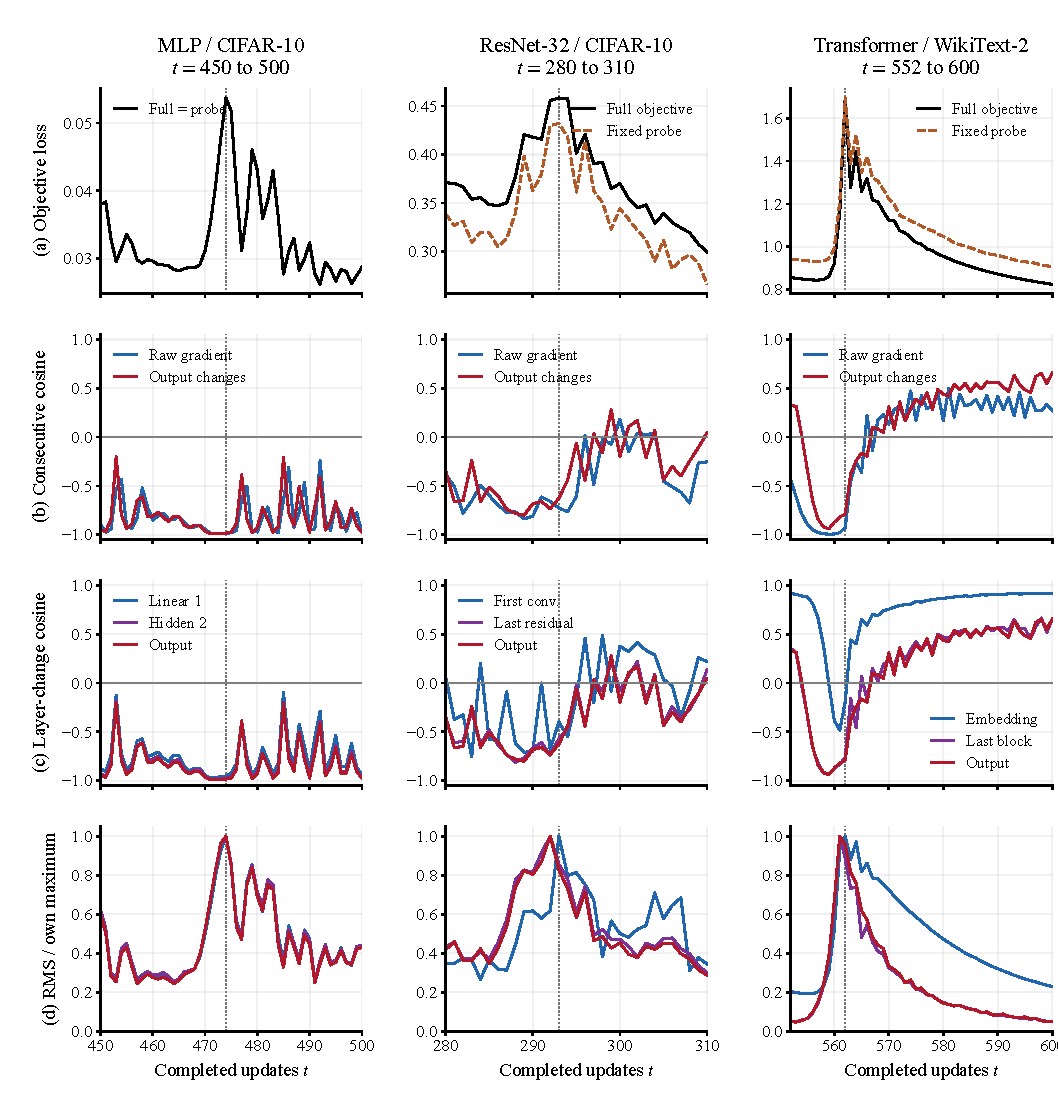
\includegraphics[width=\linewidth]{figures/architecture-comparison.pdf}
\caption{\textbf{The same diagnostics, different architectural traces.}
(a) Native full-objective and fixed-probe loss.
(b) Raw-gradient and output-displacement consecutive cosine.
(c) First learned, last hidden and output representation-change cosine.
(d) Their displacement RMS divided by each stream's own window maximum;
this compares timing, not absolute scale. Colors in (d) follow (c).
Dotted lines mark maximum full-objective loss: states 474, 293 and 562.
All values are unsmoothed; output means raw values for MLP and all
log-probabilities for the other models. Only landmarks are shown here;
the companion architecture figures retain every captured boundary.}
\label{fig:comparison}
\end{figure}

Output displacement is largest at outgoing update 474 for the MLP, but at
292 and 561 for ResNet and Transformer, respectively. Thus it can peak on
the update leaving a loss peak or on the update entering it: there is no
common ``displacement grows only after the spike'' rule. Negative cosine
also persists away from peaks, especially in the MLP. Interpret direction
together with displacement magnitude and measured loss.

\newpage
\tightsection{6. MLP: every learned representation, steps 450--500}
\begin{figure}[H]
\centering
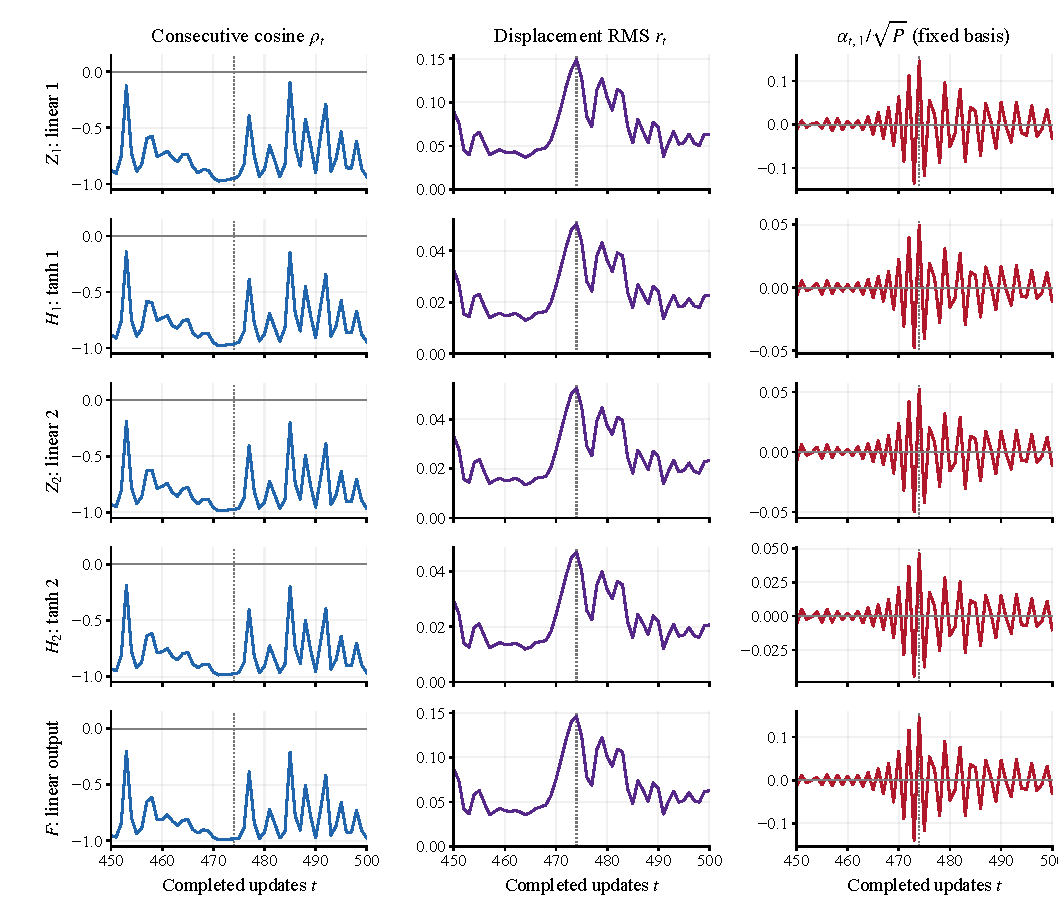
\includegraphics[width=\linewidth]{figures/mlp-layer-detail.pdf}
\caption{\textbf{A fresh fixed-window fit across the requested MLP event.}
Rows follow $Z_1=XW_1+b_1$, $H_1=\tanh Z_1$, $Z_2=H_1W_2+b_2$,
$H_2=\tanh Z_2$, and $F=H_2W_3+b_3$.
The columns show direction, absolute displacement scale, and the leading signed
SVD coefficient divided by $\sqrt{P}$ (the same units as RMS).
$P=10^6$ for hidden/preactivation tensors and $50{,}000$ for outputs.
Each layer has its own fixed pattern; its largest absolute coefficient is oriented
positive once. All five leading coefficients change sign 42 times over 50
adjacent pairs. This establishes repeated reversal along each fitted pattern,
not a common spatial axis across layers or absence of rotation.}
\label{fig:mlp}
\end{figure}

\textbf{Cost and reuse.} With $S=\sum_\ell P_\ell$ and $L$ streams, adjacent
statistics cost $O(S)$ per state; dense FP32 capture costs about $4(T+2)S$ bytes.
Exact Grams cost $O(T^2S)$, followed by $O(LT^3)$ eigendecomposition, in addition
to training and probe forwards. Original capture plus reduction took 24.9/12.6
minutes for ResNet/Transformer on one RTX 4090, with 161.8/37.6 GB derived caches;
these are whole-worker timings, not isolated overhead. This report reuses
retained Grams and requires no new training.

\textbf{Evidence.} MLP sources are Runs 240--242 and Analysis 062;
the other cases use Run 243. MLP replay is exactly qualified;
ResNet matches all 56 historical loss/norm pairs. Transformer is a qualified
continuation, not bitwise historical replay (maximum relative loss difference
0.270\% over 58 states). Analysis 063 retains source hashes, exact Gram checks
and numerical tables. Scripts \texttt{07\_mlp\_event\_window.py} and
\texttt{08\_report\_assets.py} regenerate this report's reductions and figures;
\texttt{09\_build\_report.py} compiles and checks the PDF.
The reusable protocol is \path{research/INSTABILITY_TRACING.md}.
Matched causal interventions remain a separate TODO.

\end{document}
